
\chapter{Dataset Construction}
\phantomsection
\label{ch:dataset}
\section{Khmer Text Data Collection}
\label{sec:text-source}

The dataset collection process began with gathering Khmer word-by-word data from the 
Chuon-Nath Dictionary, which provided over 50,000 words. However, it was recognized 
that sentence-by-sentence data was also necessary for comprehensive language modeling. 
To address this, a web scraping script was developed using the BeautifulSoup library 
to collect sentence data from the website khsearch.com. This resulted in the collection 
of approximately 500,000 Khmer sentences.

Upon analyzing the collected data, it was found that there was an imbalance between 
Khmer and English language data. To address this, the Alpha-Word dataset was acquired,
which contained over 300,000 English words. Furthermore, the Google-Word dataset 
was also collected, which provided a large volume of natural language data commonly 
used on the internet. Additionally, the Hugging Face dataset was used to supplement 
the collection with more natural language data.

In total, the dataset collection process yielded over 1.5 million 
character/symbols/words/sentences, including Khmer word-by-word data, 
English word-by-word data, Khmer sentences by sentences, English 
sentences by sentences, and natural language data from the internet.


\section{Text Cleaning and Preprocessing}
\label{sec:preprocessing}
The text data collected from the Chuon-Nath Dictionary, Alpha-Word, 
and Google-Word datasets was found to be clean and required no preprocessing. 
However, the text collected from internet scraping from khsearch.com was not 
clean and required preprocessing to enhance OCR performance. The text data was 
analyzed and any uncommon links or URLs, excessive spacing, tabs, and invisible 
characters were removed. Furthermore, the sentences in the text data were found 
to be too long, so the text data was segmented into word-by-word format using the 
khmer-nltk library and then random sentences were generated from 1 to 110 
characters in length, while maintaining the order of the sentences. 
This was done to ensure that the OCR model could predict missing characters 
based on the natural order of the sentences. Additionally, the text data was 
normalized to ensure that all characters were in the same format, which is 
important for OCR performance. The normalization process involved converting 
all characters to lowercase and removing any non-alphanumeric characters. 
After preprocessing, the dataset was split into two parts: a training set 
and a validation set. The training set was used to train the OCR model, 
while the validation set was used to evaluate the performance of the OCR model.


\section{Image Generation Pipeline}
\label{sec:generation}
The synthetic dataset was generated by loading text from data\_khmer\_text.txt line 
by line and applying different fonts using the Pillow library. The aim of this 
step was to generate a wide variety of text styles and fonts, so that the OCR 
model could be trained on diverse text styles. To achieve this, approximately 
50 different font styles were applied to each line of text. Additionally, 
each line was combined with 20 different background images to simulate real-world 
image text. This was done to ensure that the OCR model could recognize text 
regardless of the background of the image.

Various types of noise were applied to the text images to simulate real-world 
conditions. This included gaussian blurring, dilation and erosion, blob noise, 
speckle noise, multi-scale noisy backgrounds, random concatenation of augmented 
images, and salt-paper noise. The text on the images was rotated from -3 to 3 
degrees to simulate variations in text orientation. Additionally, margins of 
1-5 pixels were randomly added to the text images to account for inconsistent 
text detection. As each text line could generate two images, the total number 
of images produced was 3 million.

\begin{figure}[ht]
    \centering
    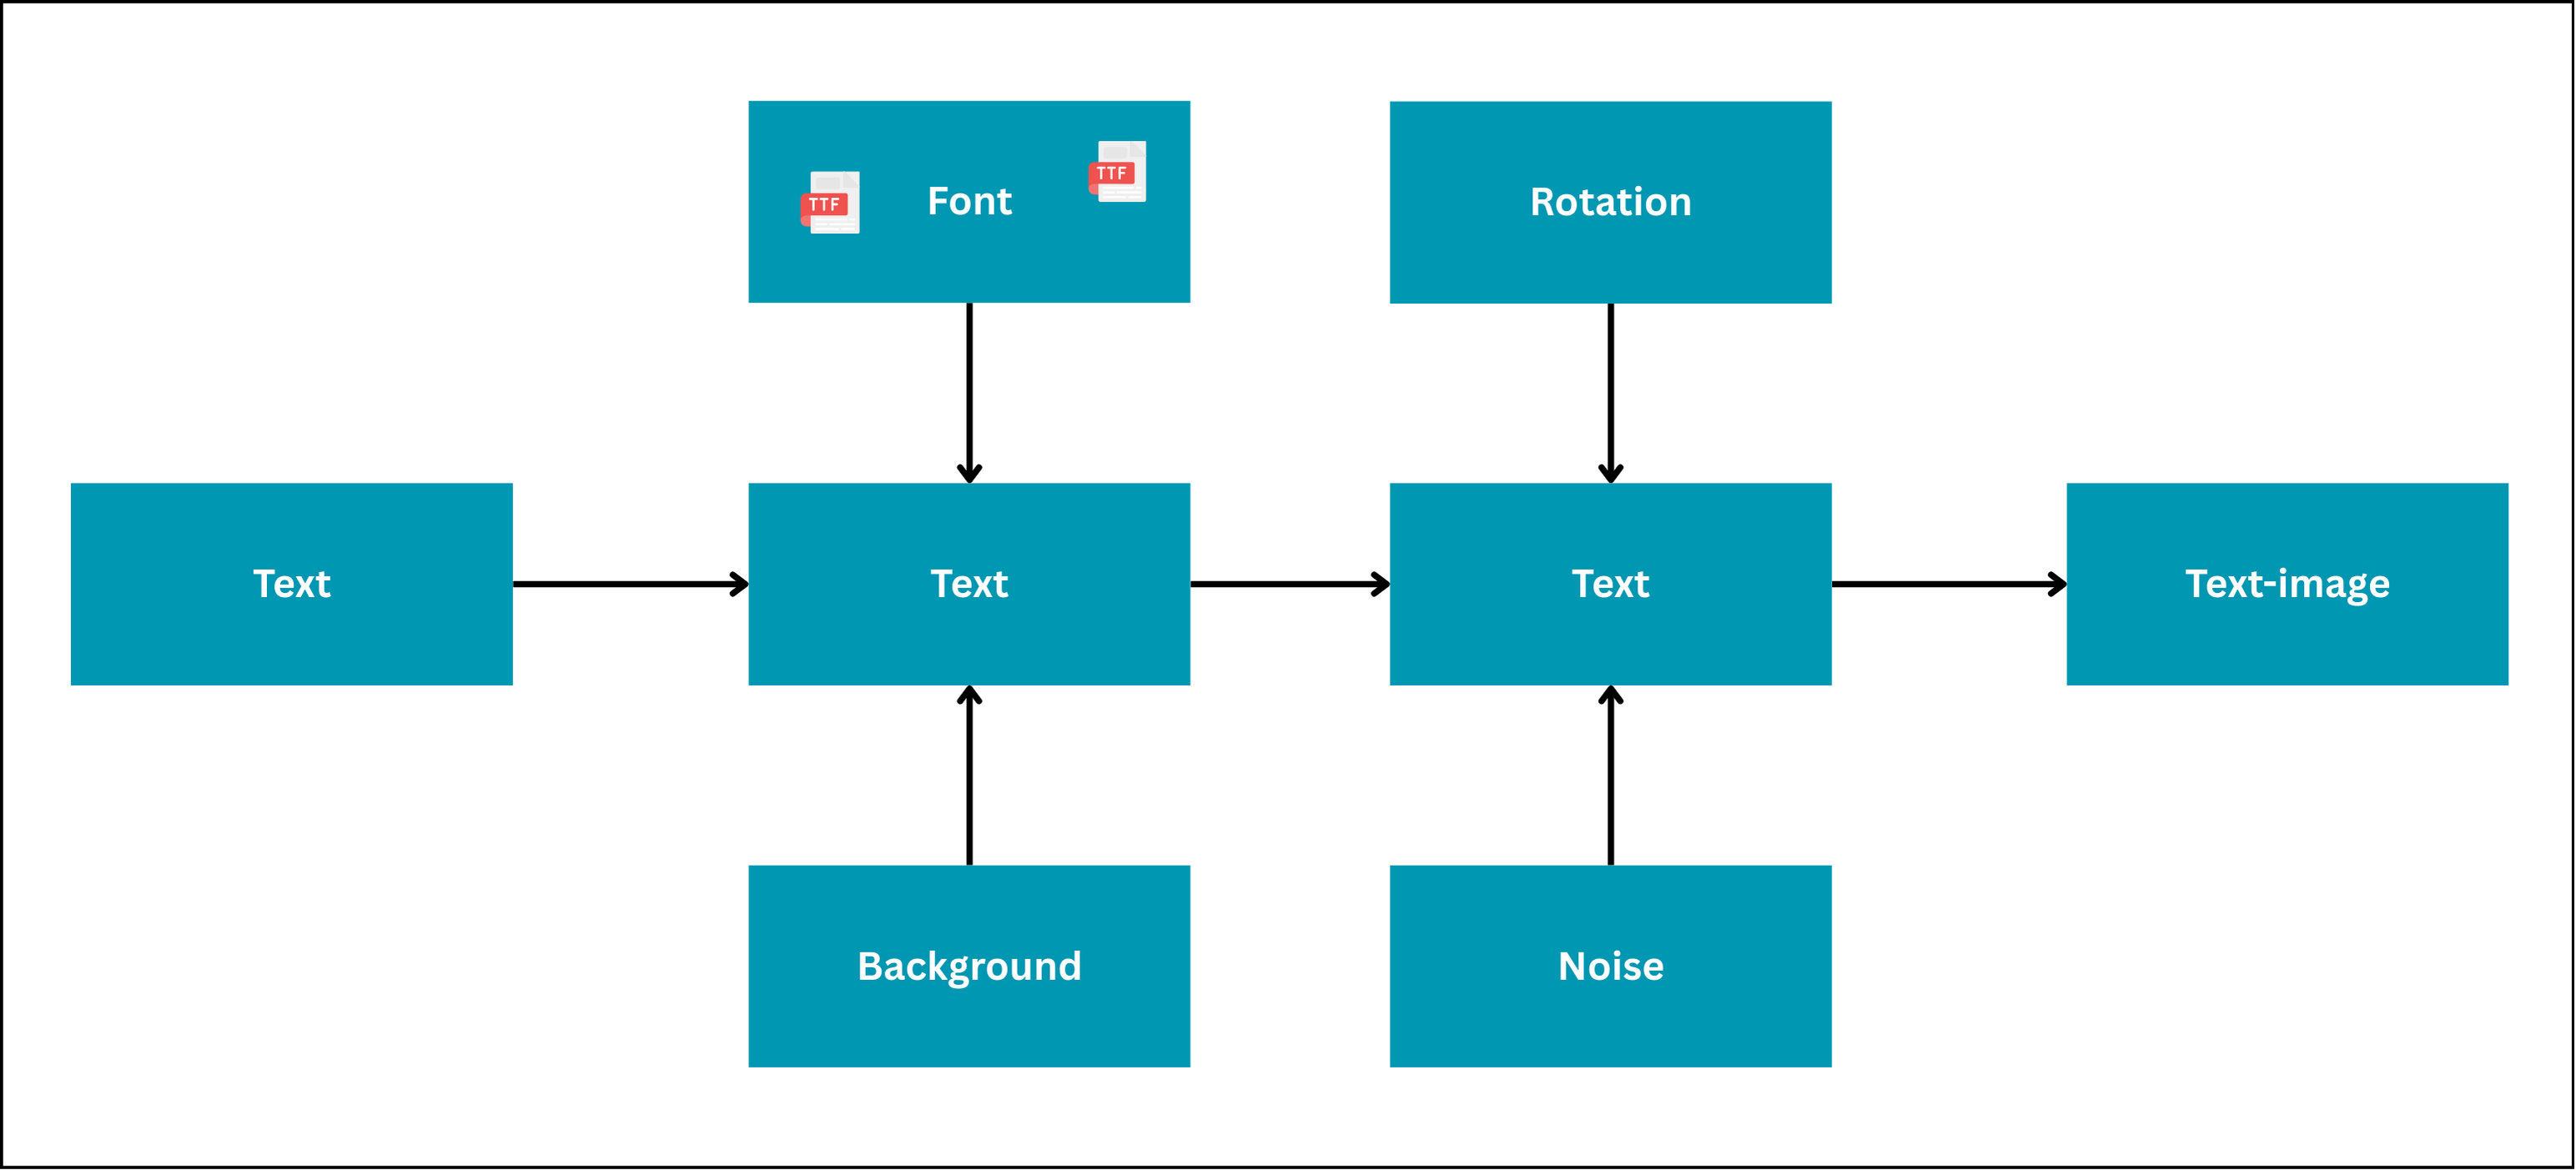
\includegraphics[width=\textwidth]{figures/synthetic_image.png}
    \caption{Example of a synthetic image generated for the OCR training dataset, 
    illustrating the application of random fonts, backgrounds, and noise to simulate 
    real-world conditions.}
    \label{fig:synthetic-image}
\end{figure}

The resulting synthetic dataset contained 3 million images, each with a unique 
combination of font, background, and noise. The images were designed to simulate 
real-world conditions, such as text orientation, text margins, and various types of 
noise. The application of these techniques resulted in a high-quality synthetic dataset 
that was suitable for training the OCR model. When examining the resulting synthetic 
dataset, it is clear that the images are highly diverse and realistic, with a wide range 
of font styles, colors, and backgrounds. Additionally, the noise types and levels are 
varied, which will help to improve the robustness of the OCR model when trained on 
this dataset. It is also clear that the images are of high quality, with crisp and clear 
text and minimal artifacts. The overall quality of the dataset is high, which will help 
to ensure that the OCR model is well-trained and can accurately recognize text in a 
variety of contexts.

\begin{figure}[ht]
    \centering
    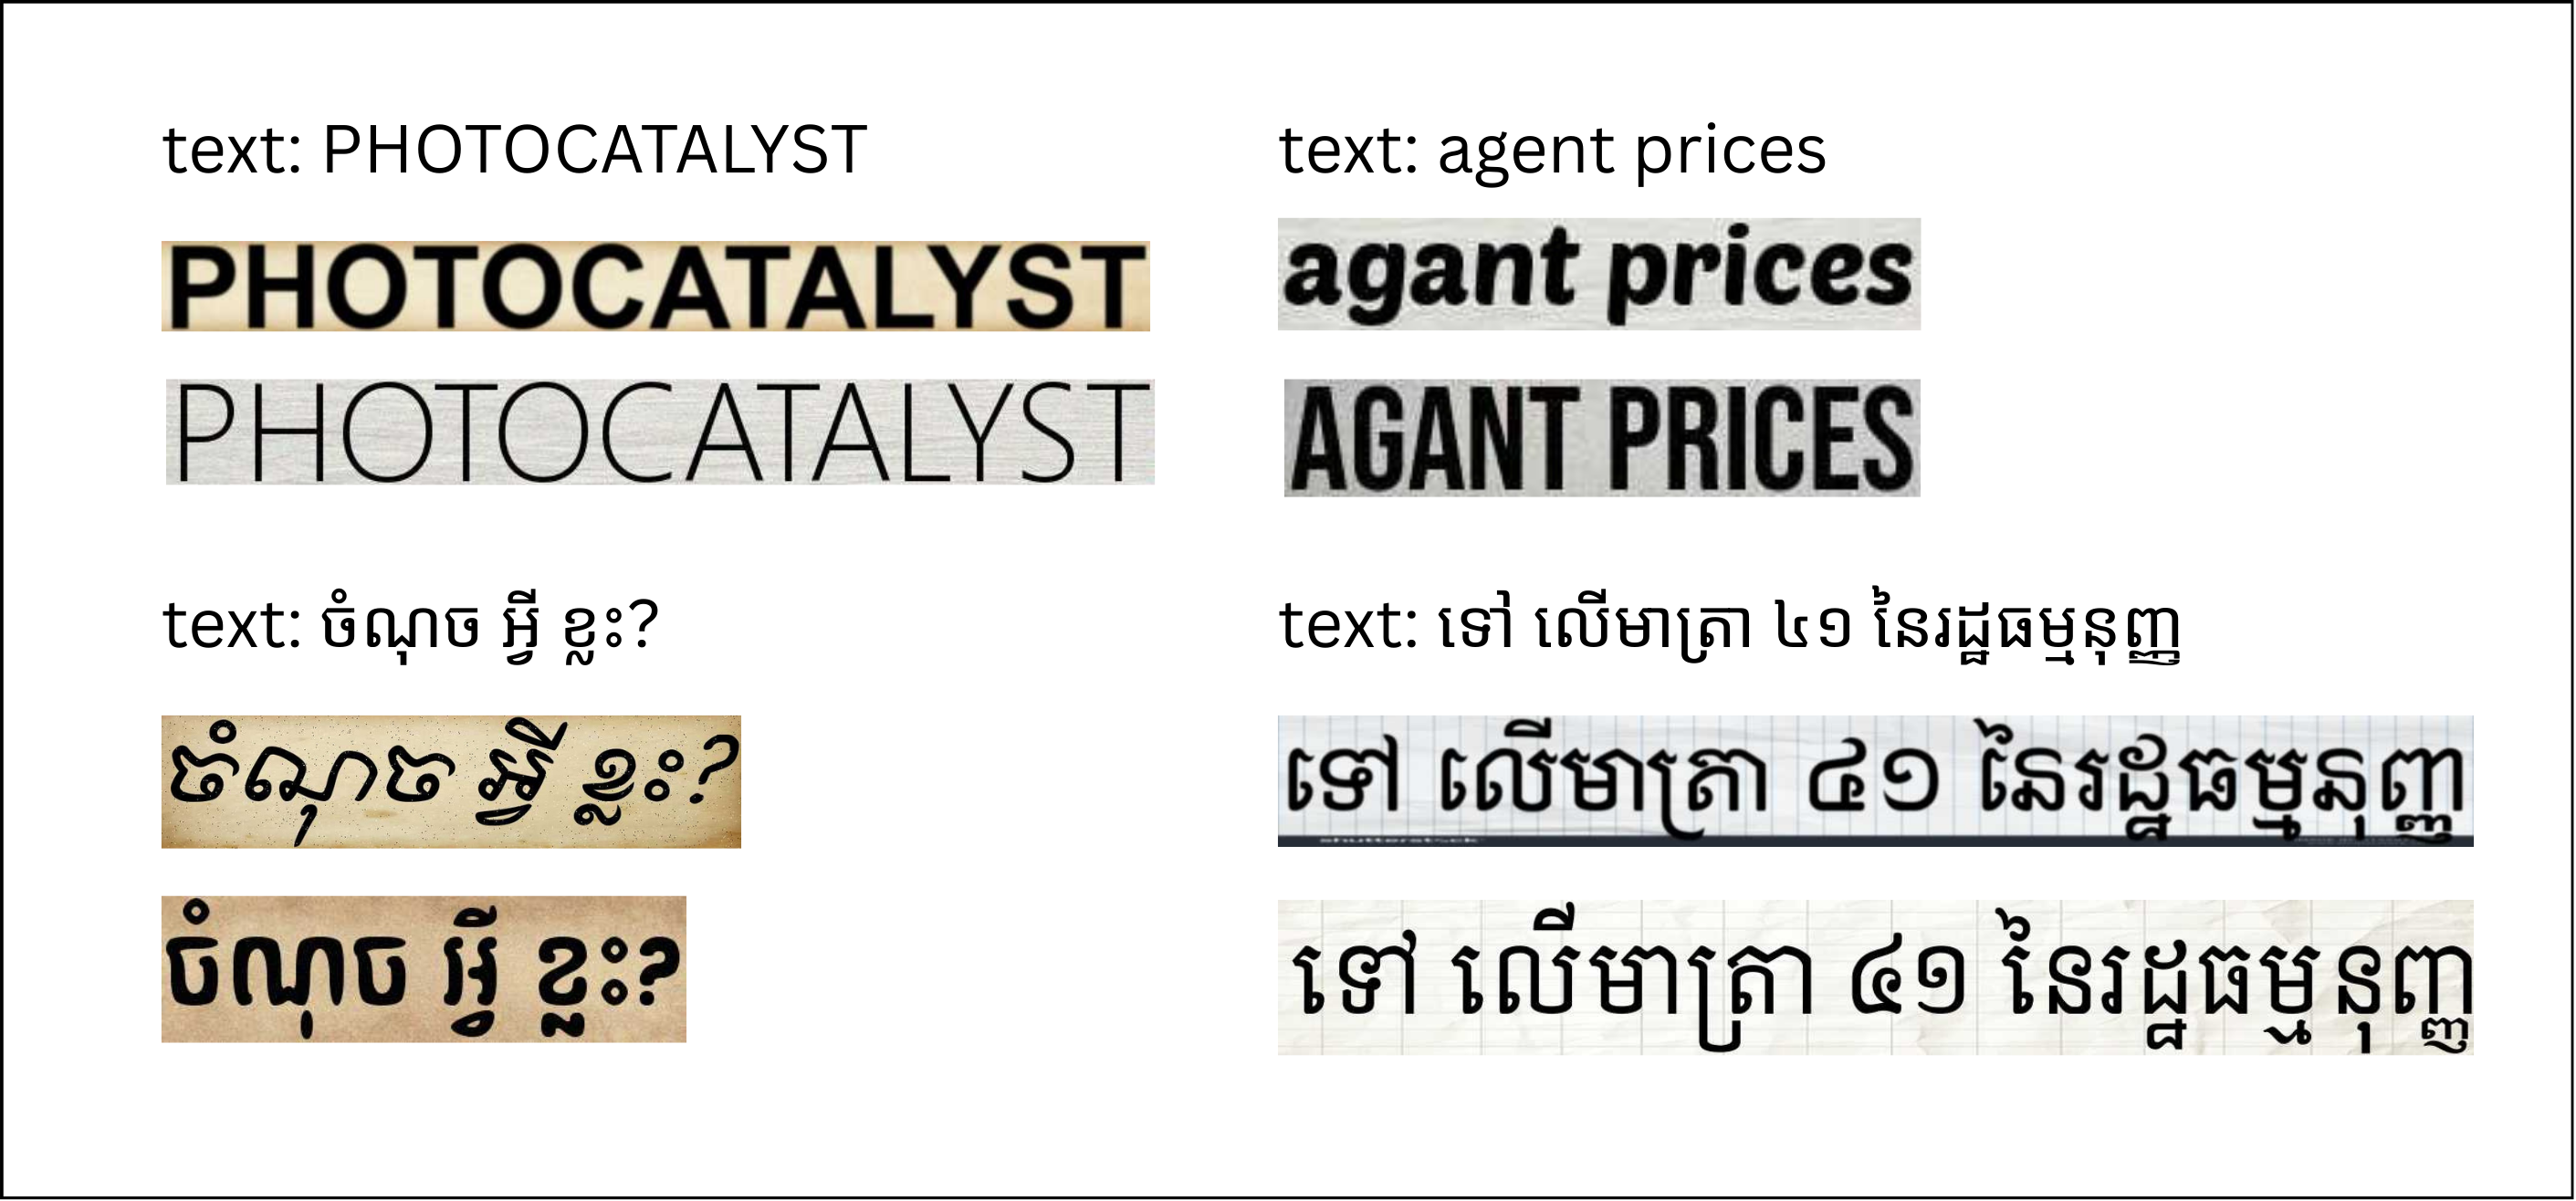
\includegraphics[width=\textwidth]{figures/resutl_synthetic_dataset.png}
    \caption{Result of the synthetic dataset generation pipeline, showing the diversity of fonts, backgrounds, and noise types.}
    \label{fig:result_synthetic_dataset}
\end{figure}

\begin{figure}[ht]
    \centering
    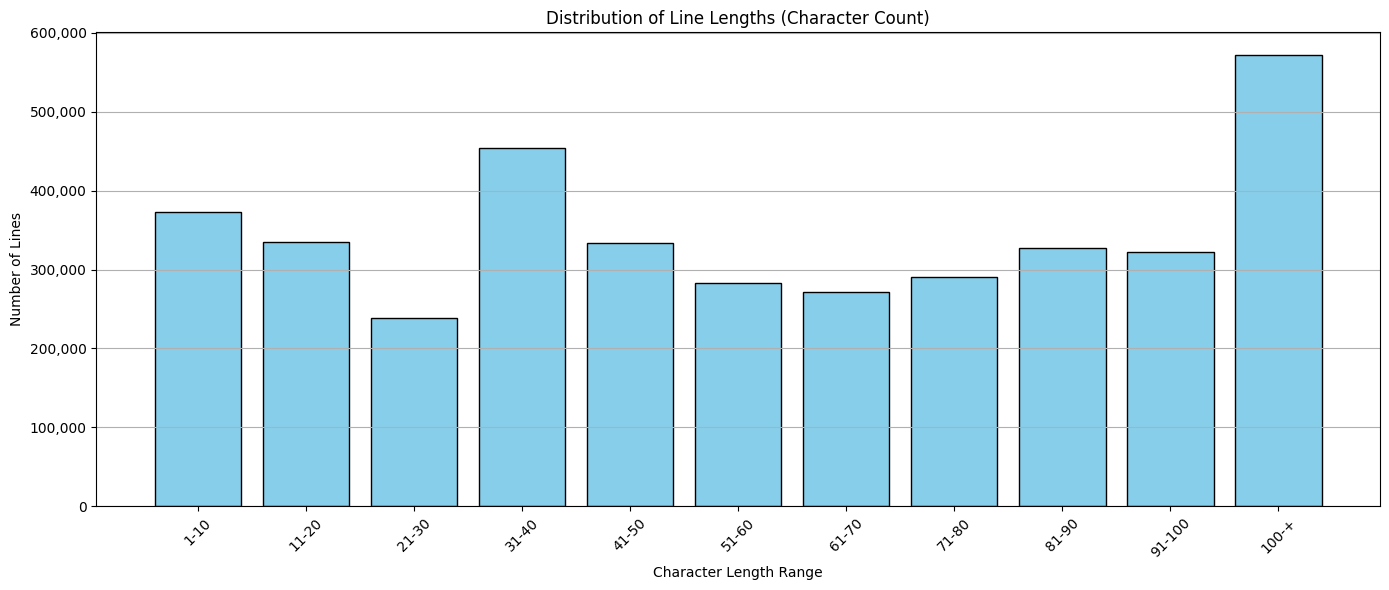
\includegraphics[width=\textwidth]{figures/frequency_of_text_length.png}
    \caption{Frequency of text length in the synthetic dataset, 
    showing the distribution of text lengths. The majority of the text  
    lengths are between 1-50 characters, with a peak at around 20-30 characters. 
    The longer text lengths are less frequent, but still present in the dataset.}
    \label{fig:frequency_of_text_length}
\end{figure}
